% TikZ/PGFPlots figure: Birkhoff Uniformity Collapse
% Usage: % TikZ/PGFPlots figure: Birkhoff Uniformity Collapse
% Usage: % TikZ/PGFPlots figure: Birkhoff Uniformity Collapse
% Usage: % TikZ/PGFPlots figure: Birkhoff Uniformity Collapse
% Usage: \input{figures/birkhoff_collapse} inside a figure environment
%
% Shows variance retention (%) vs cycle k for:
%   - Sinkhorn n=50 (collapses to 0% by cycle 10)
%   - Sinkhorn n=10 (collapses to 0% by cycle 6)
%   - SpectralSphere+residual n=50 (stable at 142%)
%   - SpectralSphere+residual n=10 (stable at 20%)

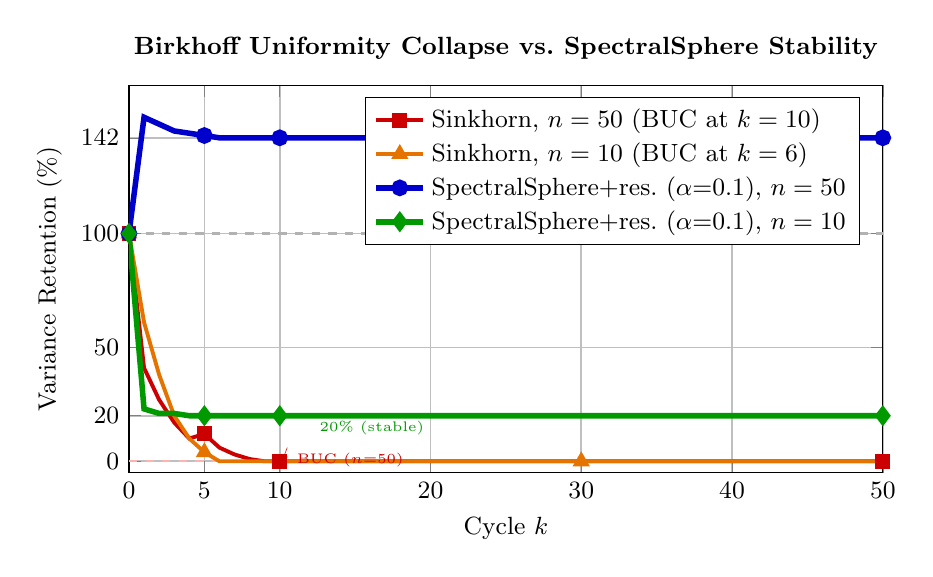
\begin{tikzpicture}
  \begin{axis}[
    width=0.92\linewidth,
    height=6.5cm,
    xlabel={Cycle $k$},
    ylabel={Variance Retention (\%)},
    xmin=0, xmax=50,
    ymin=-5, ymax=165,
    xtick={0,5,10,20,30,40,50},
    ytick={0,20,50,100,142},
    yticklabels={0, 20, 50, 100, 142},
    grid=both,
    grid style={line width=0.3pt, draw=gray!30},
    major grid style={line width=0.6pt, draw=gray!50},
    legend pos=north east,
    legend style={font=\small, cells={anchor=west}},
    tick label style={font=\small},
    label style={font=\small},
    title style={font=\small\bfseries},
    title={Birkhoff Uniformity Collapse vs.\ SpectralSphere Stability},
    clip=true,
  ]

  %% Reference lines
  \draw[dashed, gray!60, line width=0.8pt] (axis cs:0,100) -- (axis cs:50,100)
    node[right, font=\tiny, gray] {100\%};
  \draw[dashed, red!30, line width=0.8pt] (axis cs:0,0) -- (axis cs:50,0);

  %% Sinkhorn n=50: collapses by cycle 10
  \addplot[
    color=red!80!black,
    line width=1.4pt,
    mark=square*,
    mark size=2.0pt,
    mark repeat=5,
  ] coordinates {
    (0,100) (1,41) (2,27) (3,17) (4,10) (5,12) (6,6) (7,3) (8,1) (9,0)
    (10,0) (15,0) (20,0) (30,0) (40,0) (50,0)
  };
  \addlegendentry{Sinkhorn, $n=50$ (BUC at $k=10$)}

  %% Sinkhorn n=10: collapses faster, by cycle 6
  \addplot[
    color=orange!90!black,
    line width=1.4pt,
    mark=triangle*,
    mark size=2.2pt,
    mark repeat=5,
  ] coordinates {
    (0,100) (1,61) (2,38) (3,20) (4,10) (5,4) (6,0)
    (10,0) (15,0) (20,0) (30,0) (40,0) (50,0)
  };
  \addlegendentry{Sinkhorn, $n=10$ (BUC at $k=6$)}

  %% SpectralSphere + residual n=50: stable at 142%
  \addplot[
    color=blue!80!black,
    line width=2.0pt,
    mark=*,
    mark size=2.0pt,
    mark repeat=5,
  ] coordinates {
    (0,100) (1,151) (2,148) (3,145) (4,144) (5,143) (6,142) (7,142)
    (8,142) (9,142) (10,142) (15,142) (20,142) (30,142) (40,142) (50,142)
  };
  \addlegendentry{SpectralSphere+res.\ ($\alpha{=}0.1$), $n=50$}

  %% SpectralSphere + residual n=10: stable at 20%
  \addplot[
    color=green!60!black,
    line width=2.0pt,
    mark=diamond*,
    mark size=2.2pt,
    mark repeat=5,
  ] coordinates {
    (0,100) (1,23) (2,21) (3,21) (4,20) (5,20) (6,20) (7,20)
    (8,20) (9,20) (10,20) (15,20) (20,20) (30,20) (40,20) (50,20)
  };
  \addlegendentry{SpectralSphere+res.\ ($\alpha{=}0.1$), $n=10$}

  %% Annotation: collapse point n=50
  \node[font=\tiny, red!80!black, anchor=north west] at (axis cs:10.5,8)
    {BUC ($n{=}50$)};
  \draw[->, red!80!black, very thin] (axis cs:10.5,6) -- (axis cs:10.2,1);

  %% Annotation: stable equilibrium n=50
  \node[font=\tiny, blue!80!black, anchor=south west] at (axis cs:20,143)
    {$142\%$ (stable)};

  %% Annotation: stable equilibrium n=10
  \node[font=\tiny, green!60!black, anchor=north west] at (axis cs:12,22)
    {$20\%$ (stable)};

  \end{axis}
\end{tikzpicture}
 inside a figure environment
%
% Shows variance retention (%) vs cycle k for:
%   - Sinkhorn n=50 (collapses to 0% by cycle 10)
%   - Sinkhorn n=10 (collapses to 0% by cycle 6)
%   - SpectralSphere+residual n=50 (stable at 142%)
%   - SpectralSphere+residual n=10 (stable at 20%)

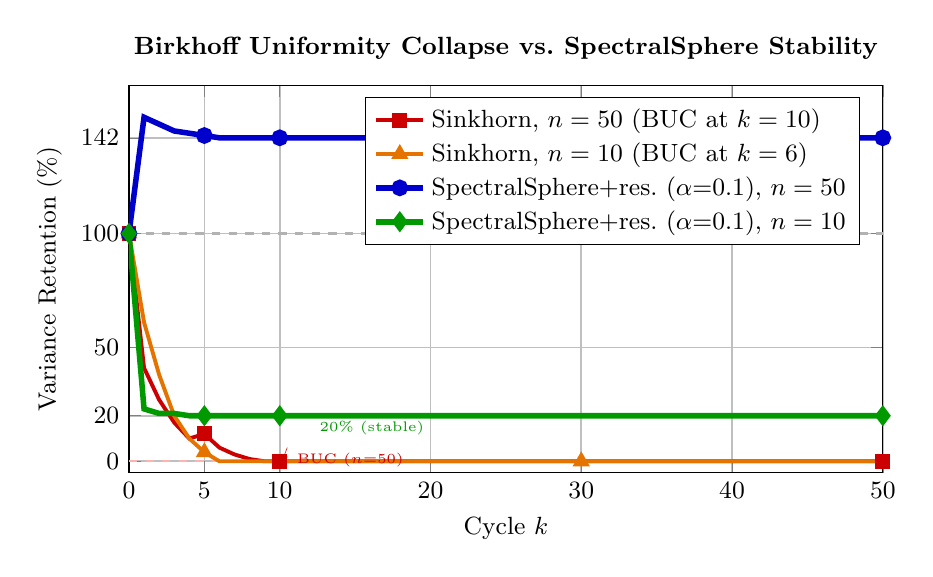
\begin{tikzpicture}
  \begin{axis}[
    width=0.92\linewidth,
    height=6.5cm,
    xlabel={Cycle $k$},
    ylabel={Variance Retention (\%)},
    xmin=0, xmax=50,
    ymin=-5, ymax=165,
    xtick={0,5,10,20,30,40,50},
    ytick={0,20,50,100,142},
    yticklabels={0, 20, 50, 100, 142},
    grid=both,
    grid style={line width=0.3pt, draw=gray!30},
    major grid style={line width=0.6pt, draw=gray!50},
    legend pos=north east,
    legend style={font=\small, cells={anchor=west}},
    tick label style={font=\small},
    label style={font=\small},
    title style={font=\small\bfseries},
    title={Birkhoff Uniformity Collapse vs.\ SpectralSphere Stability},
    clip=true,
  ]

  %% Reference lines
  \draw[dashed, gray!60, line width=0.8pt] (axis cs:0,100) -- (axis cs:50,100)
    node[right, font=\tiny, gray] {100\%};
  \draw[dashed, red!30, line width=0.8pt] (axis cs:0,0) -- (axis cs:50,0);

  %% Sinkhorn n=50: collapses by cycle 10
  \addplot[
    color=red!80!black,
    line width=1.4pt,
    mark=square*,
    mark size=2.0pt,
    mark repeat=5,
  ] coordinates {
    (0,100) (1,41) (2,27) (3,17) (4,10) (5,12) (6,6) (7,3) (8,1) (9,0)
    (10,0) (15,0) (20,0) (30,0) (40,0) (50,0)
  };
  \addlegendentry{Sinkhorn, $n=50$ (BUC at $k=10$)}

  %% Sinkhorn n=10: collapses faster, by cycle 6
  \addplot[
    color=orange!90!black,
    line width=1.4pt,
    mark=triangle*,
    mark size=2.2pt,
    mark repeat=5,
  ] coordinates {
    (0,100) (1,61) (2,38) (3,20) (4,10) (5,4) (6,0)
    (10,0) (15,0) (20,0) (30,0) (40,0) (50,0)
  };
  \addlegendentry{Sinkhorn, $n=10$ (BUC at $k=6$)}

  %% SpectralSphere + residual n=50: stable at 142%
  \addplot[
    color=blue!80!black,
    line width=2.0pt,
    mark=*,
    mark size=2.0pt,
    mark repeat=5,
  ] coordinates {
    (0,100) (1,151) (2,148) (3,145) (4,144) (5,143) (6,142) (7,142)
    (8,142) (9,142) (10,142) (15,142) (20,142) (30,142) (40,142) (50,142)
  };
  \addlegendentry{SpectralSphere+res.\ ($\alpha{=}0.1$), $n=50$}

  %% SpectralSphere + residual n=10: stable at 20%
  \addplot[
    color=green!60!black,
    line width=2.0pt,
    mark=diamond*,
    mark size=2.2pt,
    mark repeat=5,
  ] coordinates {
    (0,100) (1,23) (2,21) (3,21) (4,20) (5,20) (6,20) (7,20)
    (8,20) (9,20) (10,20) (15,20) (20,20) (30,20) (40,20) (50,20)
  };
  \addlegendentry{SpectralSphere+res.\ ($\alpha{=}0.1$), $n=10$}

  %% Annotation: collapse point n=50
  \node[font=\tiny, red!80!black, anchor=north west] at (axis cs:10.5,8)
    {BUC ($n{=}50$)};
  \draw[->, red!80!black, very thin] (axis cs:10.5,6) -- (axis cs:10.2,1);

  %% Annotation: stable equilibrium n=50
  \node[font=\tiny, blue!80!black, anchor=south west] at (axis cs:20,143)
    {$142\%$ (stable)};

  %% Annotation: stable equilibrium n=10
  \node[font=\tiny, green!60!black, anchor=north west] at (axis cs:12,22)
    {$20\%$ (stable)};

  \end{axis}
\end{tikzpicture}
 inside a figure environment
%
% Shows variance retention (%) vs cycle k for:
%   - Sinkhorn n=50 (collapses to 0% by cycle 10)
%   - Sinkhorn n=10 (collapses to 0% by cycle 6)
%   - SpectralSphere+residual n=50 (stable at 142%)
%   - SpectralSphere+residual n=10 (stable at 20%)

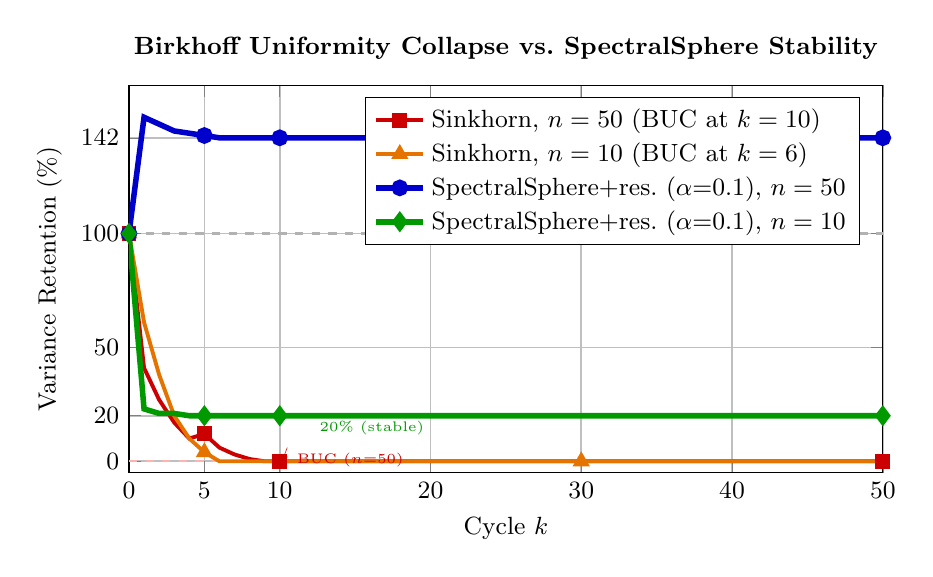
\begin{tikzpicture}
  \begin{axis}[
    width=0.92\linewidth,
    height=6.5cm,
    xlabel={Cycle $k$},
    ylabel={Variance Retention (\%)},
    xmin=0, xmax=50,
    ymin=-5, ymax=165,
    xtick={0,5,10,20,30,40,50},
    ytick={0,20,50,100,142},
    yticklabels={0, 20, 50, 100, 142},
    grid=both,
    grid style={line width=0.3pt, draw=gray!30},
    major grid style={line width=0.6pt, draw=gray!50},
    legend pos=north east,
    legend style={font=\small, cells={anchor=west}},
    tick label style={font=\small},
    label style={font=\small},
    title style={font=\small\bfseries},
    title={Birkhoff Uniformity Collapse vs.\ SpectralSphere Stability},
    clip=true,
  ]

  %% Reference lines
  \draw[dashed, gray!60, line width=0.8pt] (axis cs:0,100) -- (axis cs:50,100)
    node[right, font=\tiny, gray] {100\%};
  \draw[dashed, red!30, line width=0.8pt] (axis cs:0,0) -- (axis cs:50,0);

  %% Sinkhorn n=50: collapses by cycle 10
  \addplot[
    color=red!80!black,
    line width=1.4pt,
    mark=square*,
    mark size=2.0pt,
    mark repeat=5,
  ] coordinates {
    (0,100) (1,41) (2,27) (3,17) (4,10) (5,12) (6,6) (7,3) (8,1) (9,0)
    (10,0) (15,0) (20,0) (30,0) (40,0) (50,0)
  };
  \addlegendentry{Sinkhorn, $n=50$ (BUC at $k=10$)}

  %% Sinkhorn n=10: collapses faster, by cycle 6
  \addplot[
    color=orange!90!black,
    line width=1.4pt,
    mark=triangle*,
    mark size=2.2pt,
    mark repeat=5,
  ] coordinates {
    (0,100) (1,61) (2,38) (3,20) (4,10) (5,4) (6,0)
    (10,0) (15,0) (20,0) (30,0) (40,0) (50,0)
  };
  \addlegendentry{Sinkhorn, $n=10$ (BUC at $k=6$)}

  %% SpectralSphere + residual n=50: stable at 142%
  \addplot[
    color=blue!80!black,
    line width=2.0pt,
    mark=*,
    mark size=2.0pt,
    mark repeat=5,
  ] coordinates {
    (0,100) (1,151) (2,148) (3,145) (4,144) (5,143) (6,142) (7,142)
    (8,142) (9,142) (10,142) (15,142) (20,142) (30,142) (40,142) (50,142)
  };
  \addlegendentry{SpectralSphere+res.\ ($\alpha{=}0.1$), $n=50$}

  %% SpectralSphere + residual n=10: stable at 20%
  \addplot[
    color=green!60!black,
    line width=2.0pt,
    mark=diamond*,
    mark size=2.2pt,
    mark repeat=5,
  ] coordinates {
    (0,100) (1,23) (2,21) (3,21) (4,20) (5,20) (6,20) (7,20)
    (8,20) (9,20) (10,20) (15,20) (20,20) (30,20) (40,20) (50,20)
  };
  \addlegendentry{SpectralSphere+res.\ ($\alpha{=}0.1$), $n=10$}

  %% Annotation: collapse point n=50
  \node[font=\tiny, red!80!black, anchor=north west] at (axis cs:10.5,8)
    {BUC ($n{=}50$)};
  \draw[->, red!80!black, very thin] (axis cs:10.5,6) -- (axis cs:10.2,1);

  %% Annotation: stable equilibrium n=50
  \node[font=\tiny, blue!80!black, anchor=south west] at (axis cs:20,143)
    {$142\%$ (stable)};

  %% Annotation: stable equilibrium n=10
  \node[font=\tiny, green!60!black, anchor=north west] at (axis cs:12,22)
    {$20\%$ (stable)};

  \end{axis}
\end{tikzpicture}
 inside a figure environment
%
% Shows variance retention (%) vs cycle k for:
%   - Sinkhorn n=50 (collapses to 0% by cycle 10)
%   - Sinkhorn n=10 (collapses to 0% by cycle 6)
%   - SpectralSphere+residual n=50 (stable at 142%)
%   - SpectralSphere+residual n=10 (stable at 20%)

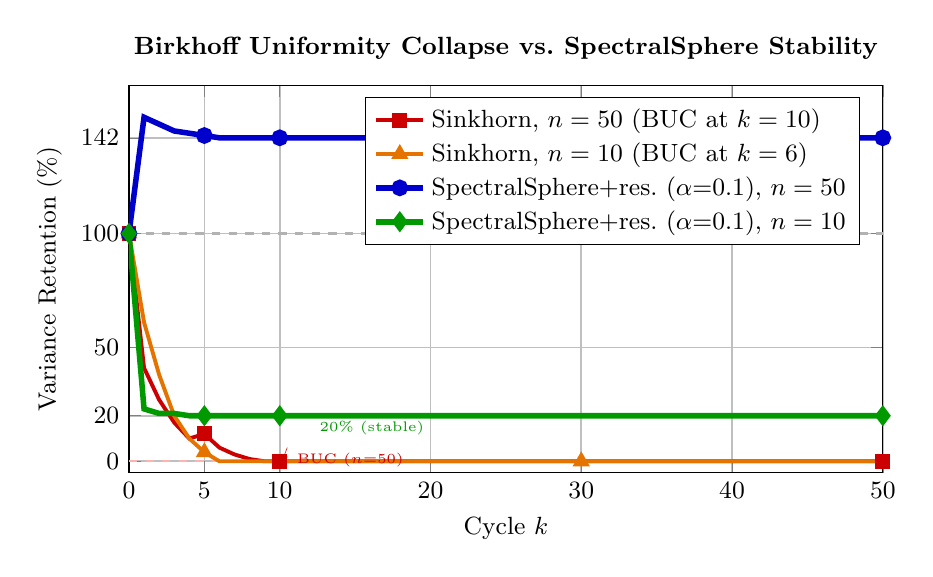
\begin{tikzpicture}
  \begin{axis}[
    width=0.92\linewidth,
    height=6.5cm,
    xlabel={Cycle $k$},
    ylabel={Variance Retention (\%)},
    xmin=0, xmax=50,
    ymin=-5, ymax=165,
    xtick={0,5,10,20,30,40,50},
    ytick={0,20,50,100,142},
    yticklabels={0, 20, 50, 100, 142},
    grid=both,
    grid style={line width=0.3pt, draw=gray!30},
    major grid style={line width=0.6pt, draw=gray!50},
    legend pos=north east,
    legend style={font=\small, cells={anchor=west}},
    tick label style={font=\small},
    label style={font=\small},
    title style={font=\small\bfseries},
    title={Birkhoff Uniformity Collapse vs.\ SpectralSphere Stability},
    clip=true,
  ]

  %% Reference lines
  \draw[dashed, gray!60, line width=0.8pt] (axis cs:0,100) -- (axis cs:50,100)
    node[right, font=\tiny, gray] {100\%};
  \draw[dashed, red!30, line width=0.8pt] (axis cs:0,0) -- (axis cs:50,0);

  %% Sinkhorn n=50: collapses by cycle 10
  \addplot[
    color=red!80!black,
    line width=1.4pt,
    mark=square*,
    mark size=2.0pt,
    mark repeat=5,
  ] coordinates {
    (0,100) (1,41) (2,27) (3,17) (4,10) (5,12) (6,6) (7,3) (8,1) (9,0)
    (10,0) (15,0) (20,0) (30,0) (40,0) (50,0)
  };
  \addlegendentry{Sinkhorn, $n=50$ (BUC at $k=10$)}

  %% Sinkhorn n=10: collapses faster, by cycle 6
  \addplot[
    color=orange!90!black,
    line width=1.4pt,
    mark=triangle*,
    mark size=2.2pt,
    mark repeat=5,
  ] coordinates {
    (0,100) (1,61) (2,38) (3,20) (4,10) (5,4) (6,0)
    (10,0) (15,0) (20,0) (30,0) (40,0) (50,0)
  };
  \addlegendentry{Sinkhorn, $n=10$ (BUC at $k=6$)}

  %% SpectralSphere + residual n=50: stable at 142%
  \addplot[
    color=blue!80!black,
    line width=2.0pt,
    mark=*,
    mark size=2.0pt,
    mark repeat=5,
  ] coordinates {
    (0,100) (1,151) (2,148) (3,145) (4,144) (5,143) (6,142) (7,142)
    (8,142) (9,142) (10,142) (15,142) (20,142) (30,142) (40,142) (50,142)
  };
  \addlegendentry{SpectralSphere+res.\ ($\alpha{=}0.1$), $n=50$}

  %% SpectralSphere + residual n=10: stable at 20%
  \addplot[
    color=green!60!black,
    line width=2.0pt,
    mark=diamond*,
    mark size=2.2pt,
    mark repeat=5,
  ] coordinates {
    (0,100) (1,23) (2,21) (3,21) (4,20) (5,20) (6,20) (7,20)
    (8,20) (9,20) (10,20) (15,20) (20,20) (30,20) (40,20) (50,20)
  };
  \addlegendentry{SpectralSphere+res.\ ($\alpha{=}0.1$), $n=10$}

  %% Annotation: collapse point n=50
  \node[font=\tiny, red!80!black, anchor=north west] at (axis cs:10.5,8)
    {BUC ($n{=}50$)};
  \draw[->, red!80!black, very thin] (axis cs:10.5,6) -- (axis cs:10.2,1);

  %% Annotation: stable equilibrium n=50
  \node[font=\tiny, blue!80!black, anchor=south west] at (axis cs:20,143)
    {$142\%$ (stable)};

  %% Annotation: stable equilibrium n=10
  \node[font=\tiny, green!60!black, anchor=north west] at (axis cs:12,22)
    {$20\%$ (stable)};

  \end{axis}
\end{tikzpicture}
